% Capitolo 6 - Model View Controller (MVC)
\chapter{Model View Controller}
\label{cap:model_view_controller}

\section{Obiettivi di apprendimento}
Al termine di questo capitolo sarai in grado di:
\begin{itemize}
    \item Comprendere i principi dei pattern architetturali
    \item Identificare i problemi delle applicazioni monolitiche
    \item Applicare il pattern MVC per separare le responsabilità
    \item Implementare Model, View e Controller in Java
    \item Progettare applicazioni manutenibili e scalabili
\end{itemize}

\section{Pattern architetturali}

Un \textbf{pattern architetturale} è una soluzione consolidata e riutilizzabile per organizzare il codice di un'applicazione software. I pattern architetturali definiscono la struttura generale del sistema e le relazioni tra i suoi componenti (come visto nel \autoref{cap:classi_oggetti_ereditarieta} per la progettazione orientata agli oggetti).

\subsection{Vantaggi dei pattern architetturali}

I pattern architetturali offrono una serie di vantaggi significativi nello sviluppo di applicazioni software complesse. Uno dei principali è la \textbf{separazione delle responsabilità}, dove ogni componente ha un ruolo ben definito e specifico, rendendo chiaro dove cercare il codice per una determinata funzionalità. Questo porta direttamente a una migliore \textbf{manutenibilità}: quando hai bisogno di apportare modifiche, queste rimangono localizzate nel componente responsabile senza impattare l'intero sistema. I pattern migliorano notevolmente la \textbf{testabilità}: componenti indipendenti e ben definiti sono molto più facili da testare in isolamento, poiché puoi creare mock e stub dei loro dipendenti. La struttura organizzata facilita anche la \textbf{riusabilità}: componenti ben definiti con responsabilità chiare possono essere riutilizzati in contesti e progetti diversi. Infine, offrono \textbf{scalabilità}: l'applicazione può crescere in modo organizzato aggiungendo nuovi componenti e nuove funzionalità senza necessità di refactoring massicio del codice esistente.

\subsection{Pattern MVC}
Il pattern \textbf{Model-View-Controller} è uno dei pattern architetturali più diffusi, particolarmente adatto per applicazioni con interfacce grafiche (vedi \autoref{cap:interfacce_grafiche}). Separa l'applicazione in tre componenti distinti con responsabilità specifiche.

\section{Problemi delle applicazioni monolitiche}

Prima di esplorare MVC, consideriamo un esempio di applicazione \textbf{monolitica}, dove tutta la logica è mescolata in un'unica classe.

\subsection{Esempio di codice BAD: applicazione monolitica}

\begin{lstlisting}
import javax.swing.*;
import java.awt.*;
import java.awt.event.ActionEvent;
import java.awt.event.ActionListener;
import java.util.ArrayList;

// CATTIVO ESEMPIO: tutto in una classe
public class TodoAppBad extends JFrame {
    // Dati (dovrebbero stare nel Model)
    private ArrayList<String> todoList = new ArrayList<>();  // vedi Capitolo ArrayList

    // Componenti GUI (dovrebbero stare nella View)
    private JTextArea txtArea;
    private JTextField txtInput;
    private JButton btnAdd;
    private JButton btnDelete;

    public TodoAppBad() {
        // Configura la finestra usando metodi ereditati da JFrame
        setTitle("Todo App - BAD DESIGN");
        setSize(400, 300);
        setDefaultCloseOperation(EXIT_ON_CLOSE);

        // Creazione GUI mischiata con logica - PROBLEMA: tutto insieme!
        JPanel panel = new JPanel(new BorderLayout());
        txtArea = new JTextArea();
        txtInput = new JTextField();
        btnAdd = new JButton("Aggiungi");
        btnDelete = new JButton("Cancella Tutto");

        // Logica applicazione mischiata con gestione eventi
        // Registra listener sul pulsante btnAdd tramite btnAdd.addActionListener()
        btnAdd.addActionListener(new ActionListener() {
            @Override
            public void actionPerformed(ActionEvent e) {
                // Ottiene il testo dal campo txtInput tramite il metodo txtInput.getText()
                String task = txtInput.getText();
                if (!task.isEmpty()) {
                    // Aggiunge alla lista todoList tramite il metodo todoList.add()
                    todoList.add(task);
                    // Chiamata al metodo aggiornaView() dell'istanza TodoAppBad
                    TodoAppBad.this.aggiornaView();
                    // Pulisce il campo txtInput tramite il metodo txtInput.setText()
                    txtInput.setText("");
                }
            }
        });

        // Lambda expression (vedi \autoref{cap:lambda_expressions}) per gestire il click
        // Registra listener sul pulsante btnDelete tramite btnDelete.addActionListener()
        btnDelete.addActionListener(e -> {
            // Cancella la lista todoList tramite il metodo todoList.clear()
            todoList.clear();
            // Chiamata al metodo aggiornaView() dell'istanza TodoAppBad
            TodoAppBad.this.aggiornaView();
        });

        // Layout - assemblaggio componenti
        JPanel topPanel = new JPanel(new BorderLayout());
        // Aggiunge componenti al pannello topPanel tramite topPanel.add()
        topPanel.add(txtInput, BorderLayout.CENTER);
        topPanel.add(btnAdd, BorderLayout.EAST);

        // Aggiunge pannelli al pannello principale tramite panel.add()
        panel.add(topPanel, BorderLayout.NORTH);
        panel.add(new JScrollPane(txtArea), BorderLayout.CENTER);
        panel.add(btnDelete, BorderLayout.SOUTH);

        // Aggiunge il pannello alla finestra tramite add() (ereditato da JFrame)
        add(panel);
    }

    // Metodo privato per aggiornare la visualizzazione
    private void aggiornaView() {
        StringBuilder sb = new StringBuilder();
        // Itera sui task nella lista todoList usando il metodo todoList.size()
        for (int i = 0; i < todoList.size(); i++) {
            // Costruisce la stringa usando sb.append() e todoList.get(i)
            sb.append((i + 1)).append(". ").append(todoList.get(i)).append("\n");
        }
        // Aggiorna il campo txtArea dell'istanza corrente tramite txtArea.setText()
        txtArea.setText(sb.toString());
    }
}
\end{lstlisting}

\subsection{Problemi identificati}
\begin{enumerate}
    \item \textbf{Accoppiamento forte}: GUI e logica sono inseparabili
    \item \textbf{Difficoltà di test}: impossibile testare la logica senza la GUI
    \item \textbf{Difficoltà di manutenzione}: modificare la GUI richiede toccare anche la logica
    \item \textbf{Riusabilità zero}: non si può riutilizzare la logica con una GUI diversa
    \item \textbf{Difficoltà di espansione}: aggiungere funzionalità complica ulteriormente il codice
\end{enumerate}

\section{Il pattern MVC}

Il pattern MVC risolve questi problemi dividendo l'applicazione in tre componenti distinti e comunicanti.

\subsection{Struttura del pattern}

\begin{figure}[h]
\centering
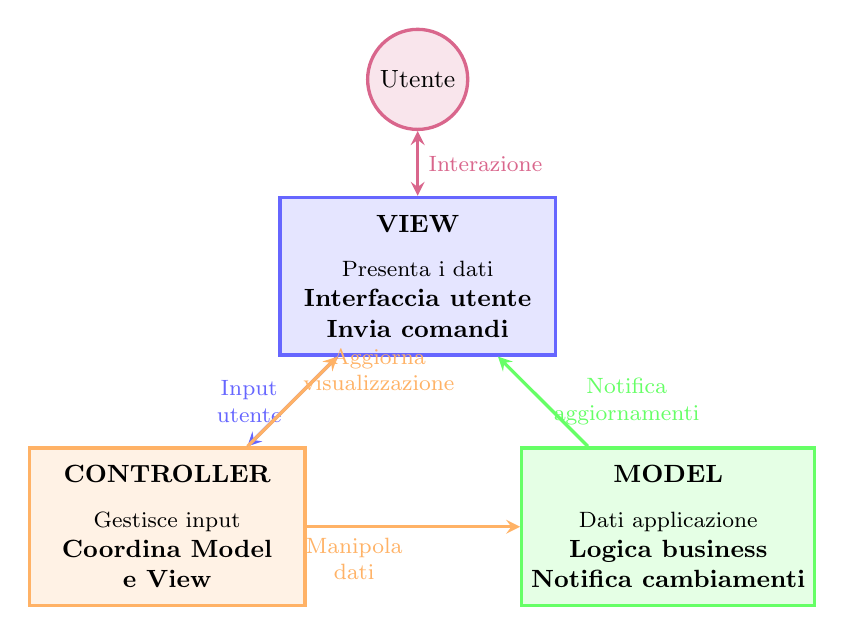
\begin{tikzpicture}[
    node distance=4cm,
    component/.style={
        rectangle,
        draw,
        very thick,
        minimum width=3.5cm,
        minimum height=2cm,
        align=center,
        font=\small\bfseries
    },
    arrow/.style={
        ->,
        >=stealth,
        very thick,
        font=\footnotesize
    }
]

% Componenti
\node[component, fill=blue!10, draw=blue!60] (view) {
    VIEW\\[5pt]
    \normalfont\footnotesize
    Presenta i dati\\
    Interfaccia utente\\
    Invia comandi
};

\node[component, fill=orange!10, draw=orange!60, below left of=view, node distance=4.5cm] (controller) {
    CONTROLLER\\[5pt]
    \normalfont\footnotesize
    Gestisce input\\
    Coordina Model\\
    e View
};

\node[component, fill=green!10, draw=green!60, below right of=view, node distance=4.5cm] (model) {
    MODEL\\[5pt]
    \normalfont\footnotesize
    Dati applicazione\\
    Logica business\\
    Notifica cambiamenti
};

% Frecce e relazioni
\draw[arrow, blue!60] (view) -- (controller) node[midway, left, align=center] {Input\\utente};
\draw[arrow, orange!60] (controller) -- (model) node[midway, below left, align=center] {Manipola\\dati};
\draw[arrow, green!60] (model) -- (view) node[midway, right, align=center] {Notifica\\aggiornamenti};
\draw[arrow, orange!60] (controller) -- (view) node[midway, above right, align=center] {Aggiorna\\visualizzazione};

% Utente
\node[circle, draw=purple!60, fill=purple!10, very thick, minimum size=1.2cm, above of=view, node distance=2.5cm, font=\small] (user) {Utente};
\draw[arrow, purple!60, <->] (user) -- (view) node[midway, right, align=left, font=\footnotesize] {Interazione};

\end{tikzpicture}
\caption{Pattern MVC: il Controller coordina le interazioni tra Model (dati) e View (interfaccia), garantendo separazione delle responsabilità}
\label{fig:pattern_mvc}
\end{figure}

\subsection{Model}
Il \textbf{Model} rappresenta i dati e la logica di business dell'applicazione. È il componente che gestisce le informazioni e le regole di business, indipendentemente dalla rappresentazione visuale.

\textbf{Responsabilità del Model}: Il Model è responsabile di gestire lo stato dell'applicazione, cioè i dati che rappresentano lo stato corrente del sistema. Deve inoltre implementare la logica di business e le regole di validazione che garantiscono che i dati rimangono in uno stato consistente. Un aspetto importante è che il Model deve notificare i cambiamenti agli osservatori (come la View) in modo che l'interfaccia utente possa aggiornarsi di conseguenza. Crucialmente, il Model non deve conoscere né la View né il Controller, mantenendosi totalmente indipendente dall'interfaccia grafica: questo permette di riutilizzare il Model in contesti completamente diversi (console, applicazioni web, applicazioni mobile, API REST) senza alcuna modifica.

\subsection{View}
La \textbf{View} è responsabile della presentazione dei dati all'utente. È il componente che gestisce l'interfaccia grafica e l'interazione con l'utente (vedi \autoref{cap:interfacce_grafiche}).

\textbf{Responsabilità della View}: La View è responsabile di visualizzare i dati del Model in modo appropriato all'utente, presentando le informazioni attraverso componenti grafici intuitivi. Deve catturare l'input dell'utente in tutte le sue forme (click di mouse, digitazione da tastiera, selection da menu, ecc.). Una responsabilità cruciale è aggiornare la visualizzazione quando il Model cambia, garantendo che l'interfaccia rimane sempre sincronizzata con lo stato attuale dell'applicazione. La View deve evitare assolutamente di contenere logica di business, limitandosi solo alla presentazione: non dovrebbe validare i dati, calcolare valori, o implementare regole di business. Infine, tutte le azioni dell'utente catturate dalla View devono essere delegate al Controller per essere gestite appropriatamente.

\subsection{Controller}
Il \textbf{Controller} fa da intermediario tra Model e View. È il componente che coordina le interazioni e gestisce il flusso dell'applicazione.

\textbf{Responsabilità del Controller}: Il Controller è responsabile di ricevere e interpretare l'input dalla View, traducendo le azioni dell'utente in comandi per il Model. Deve modificare il Model in risposta agli input dell'utente, orchestrando le operazioni necessarie. Un ruolo importante è aggiornare la View quando necessario dopo che il Model è stato modificato, garantendo che l'interfaccia rimane sincronizzata. Il Controller funge da coordinatore delle interazioni tra Model e View, gestendo il flusso di comunicazione tra i due. È importante notare che il Controller gestisce solo la logica di controllo del flusso (quali operazioni eseguire e in quale ordine), non la logica di business vera e propria, che rimane nel Model. A differenza del Model che deve essere isolato dall'interfaccia, il Controller può e deve conoscere sia il Model che la View per coordinarli effettivamente.

\section{Esempio pratico: TodoList MVC}

Implementiamo l'applicazione Todo seguendo il pattern MVC. Vedremo come separare i dati (Model), l'interfaccia grafica (View) e la logica di controllo (Controller) in tre classi distinte e ben definite.

\subsection{TodoModel: il Model}

Il Model gestisce i dati dell'applicazione utilizzando una \texttt{ArrayList<String>} per memorizzare i task (vedi \autoref{cap:arraylist} per i dettagli sulle ArrayList). Implementa anche la logica di validazione dei dati.

\begin{lstlisting}
import java.util.ArrayList;
import java.util.List;

// MODEL: contiene i dati e la logica di business
// Il Model è completamente indipendente dall'interfaccia grafica
public class TodoModel {
    // Lista dei task - dati gestiti dal Model (vedi Capitolo ArrayList)
    private List<String> todoList;

    // Costruttore: inizializza la lista todoList dell'istanza
    public TodoModel() {
        // Crea una nuova ArrayList e la assegna a todoList
        this.todoList = new ArrayList<>();
    }

    // Aggiunge un task alla lista del Model
    public boolean addTask(String task) {
        if (task == null || task.trim().isEmpty()) {
            return false; // Validazione
        }
        // Aggiunge alla lista todoList dell'istanza corrente
        this.todoList.add(task.trim());
        return true;
    }

    // Rimuove un task dalla lista del Model
    public boolean removeTask(int index) {
        if (index >= 0 && index < this.todoList.size()) {
            // Rimuove dalla lista todoList dell'istanza corrente
            this.todoList.remove(index);
            return true;
        }
        return false;
    }

    // Cancella tutti i task dal Model
    public void clearAll() {
        // Svuota la lista todoList dell'istanza corrente
        this.todoList.clear();
    }

    // Restituisce tutti i task del Model
    public List<String> getAllTasks() {
        // Restituisce una copia della lista todoList per proteggere l'incapsulamento
        return new ArrayList<>(this.todoList);
    }

    // Restituisce il numero di task nel Model
    public int getTaskCount() {
        return this.todoList.size();
    }

    // Verifica se la lista del Model è vuota
    public boolean isEmpty() {
        return this.todoList.isEmpty();
    }
}
\end{lstlisting}

\subsection{TodoView: la View}

La View gestisce l'interfaccia grafica usando componenti Swing (vedi \autoref{cap:interfacce_grafiche}). Espone metodi per visualizzare i dati e catturare l'input dell'utente, ma non contiene logica di business.

\begin{lstlisting}
import javax.swing.*;
import java.awt.*;
import java.util.List;

// VIEW: gestisce la presentazione e cattura input dell'utente
// La View contiene solo componenti grafici e metodi di visualizzazione
public class TodoView extends JFrame {
    // Componenti grafici della View
    private JTextArea txtArea;      // Area per visualizzare i task
    private JTextField txtInput;    // Campo per inserire nuovi task
    private JButton btnAdd;         // Pulsante per aggiungere task
    private JButton btnDelete;      // Pulsante per eliminare task
    private JButton btnClear;       // Pulsante per cancellare tutti i task

    public TodoView() {
        // Configura la finestra della View
        setTitle("Todo List - MVC Pattern");
        setSize(450, 350);
        setDefaultCloseOperation(JFrame.EXIT_ON_CLOSE);
        setLocationRelativeTo(null);

        // Chiama il metodo inizializzaComponenti() dell'istanza corrente
        this.inizializzaComponenti();
    }

    private void inizializzaComponenti() {
        // Area di testo per visualizzare i task
        this.txtArea = new JTextArea();
        this.txtArea.setEditable(false);
        this.txtArea.setFont(new Font("Monospaced", Font.PLAIN, 14));

        // Campo di input per nuovi task
        this.txtInput = new JTextField();

        // Pulsanti
        this.btnAdd = new JButton("Aggiungi Task");
        this.btnDelete = new JButton("Elimina Selezionato");
        this.btnClear = new JButton("Cancella Tutto");

        // Layout - organizzazione componenti grafici
        JPanel topPanel = new JPanel(new BorderLayout());
        // Imposta bordo del pannello tramite topPanel.setBorder()
        topPanel.setBorder(BorderFactory.createEmptyBorder(5, 5, 5, 5));
        // Aggiunge componenti al pannello tramite topPanel.add()
        topPanel.add(new JLabel("Nuovo Task:"), BorderLayout.WEST);
        topPanel.add(this.txtInput, BorderLayout.CENTER);
        topPanel.add(this.btnAdd, BorderLayout.EAST);

        JPanel bottomPanel = new JPanel(new FlowLayout());
        // Aggiunge pulsanti al pannello tramite bottomPanel.add()
        bottomPanel.add(this.btnDelete);
        bottomPanel.add(this.btnClear);

        // Imposta il layout della finestra tramite setLayout() (ereditato da JFrame)
        setLayout(new BorderLayout());
        // Aggiunge pannelli alla finestra tramite add() (ereditato da JFrame)
        add(topPanel, BorderLayout.NORTH);
        add(new JScrollPane(this.txtArea), BorderLayout.CENTER);
        add(bottomPanel, BorderLayout.SOUTH);
    }

    // Metodo per ottenere l'input dell'utente dal campo txtInput della View
    public String getInputTask() {
        return this.txtInput.getText();
    }

    // Pulisce il campo di input txtInput della View
    public void clearInput() {
        this.txtInput.setText("");
    }

    // Aggiorna la visualizzazione dei task nell'area txtArea della View
    public void displayTasks(List<String> tasks) {
        StringBuilder sb = new StringBuilder();
        for (int i = 0; i < tasks.size(); i++) {
            sb.append(i + 1).append(". ").append(tasks.get(i)).append("\n");
        }
        // Imposta il testo nell'area txtArea dell'istanza corrente
        this.txtArea.setText(sb.toString());
    }

    // Mostra un messaggio di errore tramite dialog della View
    public void showError(String message) {
        JOptionPane.showMessageDialog(this, message, "Errore",
                                    JOptionPane.ERROR_MESSAGE);
    }

    // Mostra un messaggio informativo tramite dialog della View
    public void showInfo(String message) {
        JOptionPane.showMessageDialog(this, message, "Informazione",
                                    JOptionPane.INFORMATION_MESSAGE);
    }

    // Metodi getter per i pulsanti della View (usati dal Controller)
    public JButton getBtnAdd() {
        return this.btnAdd;
    }

    public JButton getBtnDelete() {
        return this.btnDelete;
    }

    public JButton getBtnClear() {
        return this.btnClear;
    }
}
\end{lstlisting}

\subsection{TodoController: il Controller}

Il Controller coordina Model e View. Registra i listener per gli eventi della View e, quando l'utente interagisce con l'interfaccia, il Controller chiama i metodi appropriati del Model e della View per gestire l'azione e aggiornare la visualizzazione.

\begin{lstlisting}
import java.awt.event.ActionEvent;
import java.awt.event.ActionListener;

// CONTROLLER: coordina Model e View
// Il Controller gestisce le interazioni tra l'utente, la View e il Model
public class TodoController {
    // Riferimenti al Model e alla View gestiti da questo Controller
    private TodoModel model;
    private TodoView view;

    public TodoController(TodoModel model, TodoView view) {
        this.model = model;
        this.view = view;

        // Registra i listener per gli eventi della View
        // Ottiene i pulsanti dalla View tramite i metodi getter (view.getBtnAdd(), ecc.)
        // e assegna i listener tramite i metodi addActionListener() di ciascun pulsante
        this.view.getBtnAdd().addActionListener(new AddTaskListener());
        this.view.getBtnDelete().addActionListener(new DeleteTaskListener());
        this.view.getBtnClear().addActionListener(new ClearAllListener());

        // Aggiorna la view iniziale chiamando il metodo aggiornaView() del Controller
        this.aggiornaView();
    }

    // Listener per aggiungere un task
    class AddTaskListener implements ActionListener {
        @Override
        public void actionPerformed(ActionEvent e) {
            // Ottiene l'input dalla View tramite il metodo view.getInputTask()
            String task = view.getInputTask();

            // Aggiunge il task al Model tramite il metodo model.addTask()
            if (model.addTask(task)) {
                // Pulisce l'input della View tramite il metodo view.clearInput()
                view.clearInput();
                // Aggiorna la View chiamando il metodo aggiornaView() del Controller
                TodoController.this.aggiornaView();
            } else {
                // Mostra errore nella View tramite il metodo view.showError()
                view.showError("Inserire un task valido!");
            }
        }
    }

    // Listener per eliminare un task (non implementato completamente)
    class DeleteTaskListener implements ActionListener {
        @Override
        public void actionPerformed(ActionEvent e) {
            // Per semplicità, elimina l'ultimo task
            // Verifica se il Model è vuoto tramite il metodo model.isEmpty()
            if (!model.isEmpty()) {
                // Ottiene il numero di task dal Model con model.getTaskCount()
                // e rimuove l'ultimo tramite model.removeTask()
                model.removeTask(model.getTaskCount() - 1);
                // Aggiorna la View chiamando il metodo aggiornaView() del Controller
                TodoController.this.aggiornaView();
            } else {
                // Mostra info nella View tramite il metodo view.showInfo()
                view.showInfo("Nessun task da eliminare");
            }
        }
    }

    // Listener per cancellare tutti i task
    class ClearAllListener implements ActionListener {
        @Override
        public void actionPerformed(ActionEvent e) {
            // Verifica se il Model è vuoto tramite il metodo model.isEmpty()
            if (!model.isEmpty()) {
                // Mostra dialog di conferma
                int confirm = javax.swing.JOptionPane.showConfirmDialog(
                    view,
                    "Cancellare tutti i task?",
                    "Conferma",
                    javax.swing.JOptionPane.YES_NO_OPTION
                );

                if (confirm == javax.swing.JOptionPane.YES_OPTION) {
                    // Cancella tutti i task dal Model tramite model.clearAll()
                    model.clearAll();
                    // Aggiorna la View chiamando il metodo aggiornaView() del Controller
                    TodoController.this.aggiornaView();
                }
            }
        }
    }

    // Metodo privato del Controller per aggiornare la View con i dati del Model
    private void aggiornaView() {
        // Ottiene tutti i task dal Model tramite model.getAllTasks()
        // e aggiorna la View tramite view.displayTasks()
        view.displayTasks(model.getAllTasks());
    }
}
\end{lstlisting}

\subsection{Main: assemblaggio dell'applicazione}

\begin{lstlisting}
import javax.swing.SwingUtilities;

// MAIN: punto di ingresso dell'applicazione MVC
public class TodoApp {
    public static void main(String[] args) {
        // Esegue il codice nel thread di gestione eventi di Swing (vedi Capitolo Interfacce Grafiche)
        SwingUtilities.invokeLater(() -> {
            // Crea l'istanza del Model
            TodoModel model = new TodoModel();
            // Crea l'istanza della View
            TodoView view = new TodoView();
            // Crea l'istanza del Controller, passando Model e View
            TodoController controller = new TodoController(model, view);

            // Rende visibile la View tramite il metodo view.setVisible()
            view.setVisible(true);
        });
    }
}
\end{lstlisting}

\begin{nota}
\textbf{Principi fondamentali del pattern MVC:}
\begin{itemize}
    \item Il \textbf{Model} non conosce né View né Controller - è totalmente indipendente dall'interfaccia
    \item La \textbf{View} conosce solo le proprie componenti GUI - non contiene logica di business
    \item Il \textbf{Controller} coordina Model e View tramite i metodi pubblici di entrambi, ma non contiene logica di business
    \item La separazione permette di modificare una componente senza impattare le altre
    \item Il Model può essere testato indipendentemente senza bisogno della GUI
\end{itemize}
\end{nota}

\section{Vantaggi del pattern MVC}

Confrontando questa implementazione con l'esempio monolitico precedente:

\begin{enumerate}
    \item \textbf{Separazione netta delle responsabilità}: ogni classe ha un ruolo preciso
    \item \textbf{Testabilità}: il Model può essere testato indipendentemente dalla GUI
    \item \textbf{Manutenibilità}: modifiche alla GUI non impattano la logica
    \item \textbf{Riusabilità}: il Model può essere riutilizzato con diverse View (console, web, mobile)
    \item \textbf{Scalabilità}: l'applicazione può crescere aggiungendo funzionalità al Model
\end{enumerate}

\section{Best Practices e Errori Comuni}

Il pattern MVC è potente, ma è facile cadere in errori comuni che ne vanificano i vantaggi. In questa sezione esploriamo gli errori più frequenti e le best practices per un'implementazione corretta ed efficace del pattern.

\subsection{Errori comuni nel pattern MVC}

Ecco gli errori più diffusi che compromettono l'efficacia del pattern MVC:

\subsubsection{Logica business nella View}

\begin{lstlisting}
// ERRORE: logica di validazione nella View
public class TodoViewBad extends JFrame {
    private JButton btnAdd;

    public void setupListeners() {
        btnAdd.addActionListener(e -> {
            String task = txtInput.getText();
            // SBAGLIATO: validazione nella View!
            if (task.length() > 50) {
                showError("Task troppo lungo!");
                return;
            }
            if (task.contains("TODO")) {
                task = task.replace("TODO", "");
            }
            // Questa logica dovrebbe stare nel Model!
        });
    }
}
\end{lstlisting}

\textbf{Problema}: la View contiene logica di validazione e trasformazione dei dati, che dovrebbe essere nel Model. Questo rende impossibile riutilizzare la logica con altre interfacce.

\textbf{Soluzione corretta}: tutta la logica di validazione e business deve stare nel Model.

\subsubsection{Controller troppo voluminoso}

\begin{lstlisting}
// ERRORE: Controller con troppa logica
public class TodoControllerBad {
    public void handleAddTask() {
        String task = view.getInputTask();

        // SBAGLIATO: tutta questa logica dovrebbe stare nel Model!
        if (task == null || task.trim().isEmpty()) {
            view.showError("Task vuoto");
            return;
        }

        task = task.trim().toUpperCase(); // Trasformazione

        if (task.length() > 100) { // Validazione lunghezza
            view.showError("Task troppo lungo");
            return;
        }

        if (model.getAllTasks().contains(task)) { // Controllo duplicati
            view.showError("Task duplicato");
            return;
        }

        model.addTask(task);
        aggiornaView();
    }
}
\end{lstlisting}

\textbf{Problema}: il Controller contiene validazione, trasformazione e logica di business che dovrebbe essere delegata al Model.

\textbf{Soluzione corretta}: il Controller deve solo coordinare, non implementare logica di business.

\subsubsection{Model esposto direttamente}

\begin{lstlisting}
// ERRORE: View accede direttamente al Model
public class TodoViewBad extends JFrame {
    private TodoModel model; // SBAGLIATO: la View non deve conoscere il Model!

    public void displayTasks() {
        // SBAGLIATO: la View accede direttamente al Model
        List<String> tasks = model.getAllTasks();
        txtArea.setText(tasks.toString());
    }
}
\end{lstlisting}

\textbf{Problema}: la View accede direttamente al Model, bypassando il Controller. Questo crea accoppiamento forte e rende difficile la manutenzione.

\textbf{Soluzione corretta}: solo il Controller deve coordinare Model e View.

\subsubsection{Non separazione delle responsabilità}

\begin{lstlisting}
// ERRORE: Model che conosce la View
public class TodoModelBad {
    private TodoView view; // SBAGLIATO!

    public void addTask(String task) {
        todoList.add(task);
        view.displayTasks(todoList); // SBAGLIATO: il Model notifica la View!
    }
}
\end{lstlisting}

\textbf{Problema}: il Model dipende dalla View, rendendolo impossibile da testare e riutilizzare indipendentemente.

\textbf{Soluzione corretta}: il Model deve essere completamente indipendente dalla View e dal Controller.

\subsection{Best practices MVC}

Ecco le pratiche raccomandate per un'implementazione corretta ed efficace del pattern MVC:

\subsubsection{Single Responsibility Principle}

Ogni componente deve avere una sola responsabilità ben definita:

\begin{itemize}
    \item \textbf{Model}: gestisce SOLO dati e logica di business
    \item \textbf{View}: gestisce SOLO presentazione e cattura input
    \item \textbf{Controller}: coordina SOLO le interazioni tra Model e View
\end{itemize}

\begin{lstlisting}
// BUONA PRATICA: Model con singola responsabilità
public class TodoModel {
    private List<String> todoList;

    // Solo logica di business e gestione dati
    public boolean addTask(String task) {
        // Validazione nel Model
        if (task == null || task.trim().isEmpty()) {
            return false;
        }

        // Trasformazione nel Model
        String cleanTask = task.trim();

        // Regola di business: no duplicati
        if (todoList.contains(cleanTask)) {
            return false;
        }

        todoList.add(cleanTask);
        return true;
    }
}
\end{lstlisting}

\subsubsection{Testabilità dei componenti}

Il Model deve essere completamente testabile senza bisogno di View o Controller:

\begin{lstlisting}
// BUONA PRATICA: Model testabile indipendentemente
import org.junit.Test;
import static org.junit.Assert.*;

public class TodoModelTest {
    @Test
    public void testAddTask() {
        TodoModel model = new TodoModel();

        // Test senza GUI!
        assertTrue(model.addTask("Comprare latte"));
        assertEquals(1, model.getTaskCount());

        // Test validazione
        assertFalse(model.addTask("")); // Task vuoto
        assertFalse(model.addTask(null)); // Task null

        // Test duplicati
        assertFalse(model.addTask("Comprare latte"));
    }
}
\end{lstlisting}

\textbf{Vantaggi}: La separazione del Model dalla View fornisce numerosi vantaggi pratici. Innanzitutto, i test sono \textbf{rapidi} poiché non è necessario avviare l'intera interfaccia grafica: puoi testare la logica direttamente con semplici asserzioni. Questo porta a una \textbf{maggiore affidabilità del codice}: testare componenti in isolamento cattura i bug più efficacemente rispetto ai test dell'interfaccia grafica che sono lenti e fragili. Infine, la separazione \textbf{facilita il refactoring}: puoi modificare il Model sapendo che non stai rompendo la View, e viceversa, perché sono completamente disaccoppiati.

\subsubsection{Accoppiamento loose coupling}

Minimizzare le dipendenze tra componenti usando interfacce:

\begin{lstlisting}
// BUONA PRATICA: uso di interfacce per loose coupling
public interface ITodoModel {
    boolean addTask(String task);
    boolean removeTask(int index);
    List<String> getAllTasks();
}

public interface ITodoView {
    void displayTasks(List<String> tasks);
    String getInputTask();
    void showError(String message);
}

// Controller dipende dalle interfacce, non dalle implementazioni concrete
public class TodoController {
    private ITodoModel model;
    private ITodoView view;

    public TodoController(ITodoModel model, ITodoView view) {
        this.model = model;
        this.view = view;
    }
}
\end{lstlisting}

\textbf{Vantaggi}: L'uso di interfacce per il loose coupling offre flessibilità architettonica significativa. È \textbf{facile sostituire implementazioni} quando i requisiti cambiano: per esempio, puoi rimpiazzare una GUI sviluppata con Swing con una sviluppata in JavaFX senza toccare il Model o il Controller, perché dipendono dalla stessa interfaccia. Ciò \textbf{facilita il testing con mock objects}: puoi creare implementazioni fittizie delle interfacce che simulano il comportamento, permettendoti di testare il Controller isolatamente da Model e View reali. Globalmente, il loose coupling garantisce \textbf{maggiore flessibilità e manutenibilità}: il sistema diventa più resiliente ai cambiamenti perché le dipendenze sono gestite attraverso contratti (interfacce) anziché implementazioni concrete.

\subsubsection{Observer pattern per aggiornamenti}

Usare il pattern Observer per notificare automaticamente la View quando il Model cambia:

\begin{lstlisting}
// BUONA PRATICA: Observer pattern per aggiornamenti automatici
import java.beans.PropertyChangeListener;
import java.beans.PropertyChangeSupport;

public class TodoModelObservable {
    private List<String> todoList;
    private PropertyChangeSupport support;

    public TodoModelObservable() {
        this.todoList = new ArrayList<>();
        this.support = new PropertyChangeSupport(this);
    }

    // Metodo per registrare listener
    public void addPropertyChangeListener(PropertyChangeListener listener) {
        support.addPropertyChangeListener(listener);
    }

    public boolean addTask(String task) {
        if (task == null || task.trim().isEmpty()) {
            return false;
        }

        List<String> oldList = new ArrayList<>(todoList);
        todoList.add(task.trim());

        // Notifica automatica ai listener!
        support.firePropertyChange("todoList", oldList, new ArrayList<>(todoList));
        return true;
    }
}

// View si registra come listener
public class TodoViewObserver extends JFrame implements PropertyChangeListener {
    @Override
    public void propertyChange(PropertyChangeEvent evt) {
        if ("todoList".equals(evt.getPropertyName())) {
            // Aggiornamento automatico quando il Model cambia!
            @SuppressWarnings("unchecked")
            List<String> newTasks = (List<String>) evt.getNewValue();
            displayTasks(newTasks);
        }
    }
}
\end{lstlisting}

\textbf{Vantaggi}: L'implementazione del pattern Observer con il Model fornisce benefici significativi nell'architettura dell'applicazione. La View \textbf{si aggiorna automaticamente quando il Model cambia}, senza necessità di pull esplicito dei dati: non appena il Model modifica i dati, notifica automaticamente tutti i listener registrati. Ciò \textbf{elimina la necessità di chiamate esplicite} come \texttt{aggiornaView()}: il Controller non deve ricordarsi di aggiornare manualmente la View dopo ogni operazione sul Model. Il pattern \textbf{supporta multiple View sincronizzate sullo stesso Model}: diverse interfacce grafiche possono rimanere tutte aggiornate allo stesso stato, utile per applicazioni con viste multiple dello stesso dato. Infine, questo approccio \textbf{implementa il principio "Don't call us, we'll call you"}: la View non chiama il Model per verificare se è cambiato (polling inefficiente), ma è il Model che chiama la View per notificare i cambiamenti (push efficiente).

\subsection{Diagramma di sequenza: flusso MVC}

Il seguente diagramma mostra il flusso tipico di un'interazione nel pattern MVC con Observer pattern:

\begin{figure}[h]
\centering
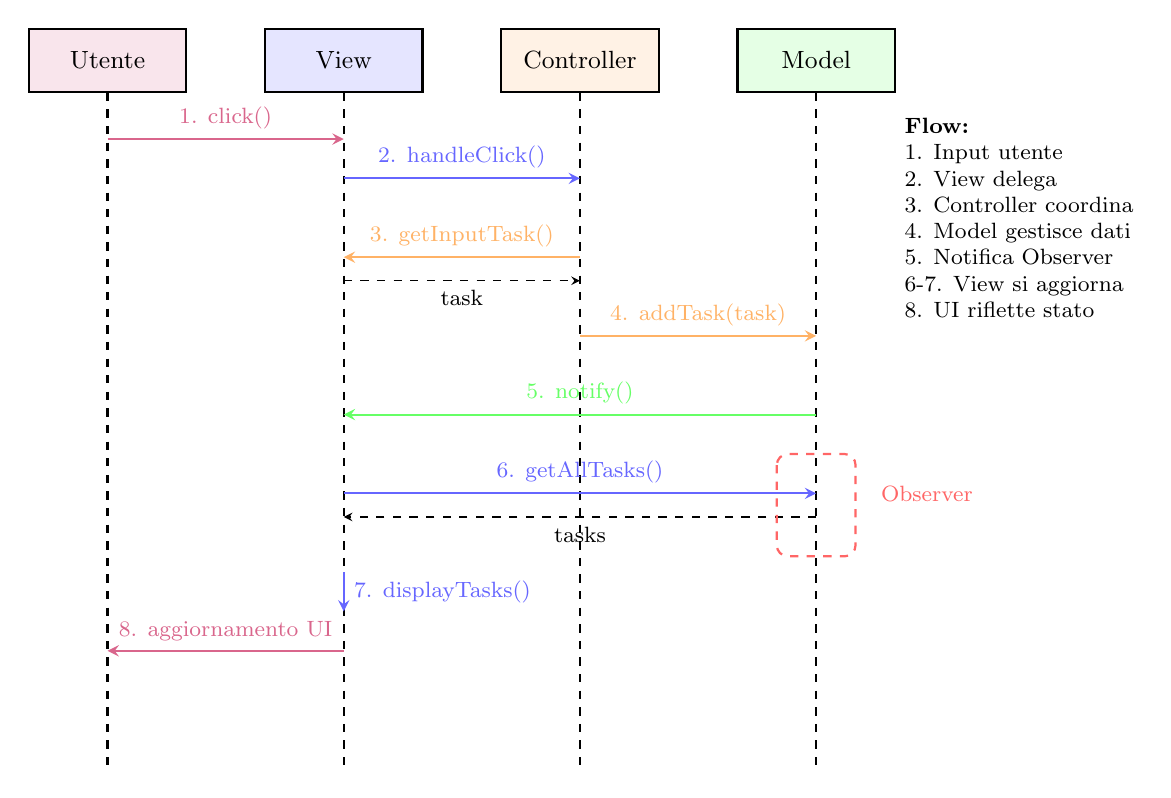
\begin{tikzpicture}[
    node distance=1.5cm,
    every node/.style={font=\small},
    box/.style={
        rectangle,
        draw,
        thick,
        minimum width=2cm,
        minimum height=0.8cm,
        align=center
    },
    lifeline/.style={
        draw,
        thick,
        dashed
    },
    message/.style={
        ->,
        >=stealth,
        thick
    },
    return/.style={
        ->,
        >=stealth,
        dashed
    }
]

% Attori/Componenti
\node[box, fill=purple!10] (user) at (0,0) {Utente};
\node[box, fill=blue!10] (view) at (3,0) {View};
\node[box, fill=orange!10] (controller) at (6,0) {Controller};
\node[box, fill=green!10] (model) at (9,0) {Model};

% Lifelines
\draw[lifeline] (user) -- (0,-9);
\draw[lifeline] (view) -- (3,-9);
\draw[lifeline] (controller) -- (6,-9);
\draw[lifeline] (model) -- (9,-9);

% Sequenza di messaggi
% 1. Click utente
\draw[message, purple!60] (0,-1) -- (3,-1) node[midway, above, font=\footnotesize] {1. click()};

% 2. View cattura evento
\draw[message, blue!60] (3,-1.5) -- (6,-1.5) node[midway, above, font=\footnotesize] {2. handleClick()};

% 3. Controller ottiene input
\draw[message, orange!60] (6,-2.5) -- (3,-2.5) node[midway, above, font=\footnotesize] {3. getInputTask()};
\draw[return] (3,-2.8) -- (6,-2.8) node[midway, below, font=\footnotesize] {task};

% 4. Controller modifica Model
\draw[message, orange!60] (6,-3.5) -- (9,-3.5) node[midway, above, font=\footnotesize] {4. addTask(task)};

% 5. Model notifica Observer
\draw[message, green!60] (9,-4.5) -- (3,-4.5) node[midway, above, font=\footnotesize] {5. notify()};

% 6. View richiede dati aggiornati
\draw[message, blue!60] (3,-5.5) -- (9,-5.5) node[midway, above, font=\footnotesize] {6. getAllTasks()};
\draw[return] (9,-5.8) -- (3,-5.8) node[midway, below, font=\footnotesize] {tasks};

% 7. View aggiorna UI
\draw[message, blue!60] (3,-6.5) -- (3,-7) node[midway, right, font=\footnotesize] {7. displayTasks()};

% 8. Feedback utente
\draw[message, purple!60] (3,-7.5) -- (0,-7.5) node[midway, above, font=\footnotesize] {8. aggiornamento UI};

% Annotazioni
\node[font=\footnotesize, align=left, anchor=west] at (10,-2) {
    \textbf{Flow:}\\
    1. Input utente\\
    2. View delega\\
    3. Controller coordina\\
    4. Model gestisce dati\\
    5. Notifica Observer\\
    6-7. View si aggiorna\\
    8. UI riflette stato
};

% Box evidenziazione Observer
\draw[draw=red!60, thick, dashed, rounded corners] (8.5,-5) rectangle (9.5,-6.3);
\node[font=\footnotesize, text=red!60, anchor=west] at (9.7,-5.5) {Observer};

\end{tikzpicture}
\caption{Diagramma di sequenza MVC con Observer pattern: il flusso mostra come l'interazione utente attraversa View, Controller e Model, con aggiornamento automatico tramite notifica Observer}
\label{fig:mvc_sequence}
\end{figure}

\textbf{Spiegazione del flusso}:
\begin{enumerate}
    \item L'utente interagisce con la View (es. click su pulsante "Aggiungi")
    \item La View cattura l'evento e lo delega al Controller tramite un listener
    \item Il Controller ottiene l'input dalla View tramite metodi getter
    \item Il Controller chiama il Model per modificare i dati
    \item Il Model notifica automaticamente tutti gli Observer registrati (inclusa la View)
    \item La View riceve la notifica e richiede i dati aggiornati al Model
    \item La View aggiorna l'interfaccia grafica con i nuovi dati
    \item L'utente vede l'aggiornamento nell'interfaccia
\end{enumerate}

\begin{nota}
\textbf{Vantaggi del flusso Observer}: L'implementazione del flusso Observer nel pattern MVC fornisce vantaggi architetturali significativi. Il Controller non deve chiamare esplicitamente \texttt{aggiornaView()} dopo ogni operazione sul Model: la notifica automatica del Model gestisce tutto. Multiple View possono rimanere sincronizzate automaticamente sullo stesso Model senza sforzi aggiuntivi di coordinamento. Il Model rimane completamente indipendente dalla View anche in questo scenario avanzato: non conosce l'esistenza della View, ma comunica solo tramite il pattern Observer. Questo approccio segue il principio Hollywood: "Don't call us, we'll call you", dove la View non interroga costantemente il Model, ma rimane in ascolto dei cambiamenti che il Model le notifica proattivamente.
\end{nota}

\section{Riepilogo}

In questo capitolo abbiamo studiato il pattern architetturale Model-View-Controller, fondamentale per la progettazione di applicazioni moderne. I \textbf{pattern architetturali} sono soluzioni consolidate e riutilizzabili per organizzare il codice delle applicazioni di grandi dimensioni. Abbiamo visto i \textbf{problemi delle applicazioni monolitiche}, dove il codice è mescolato in una singola classe, causando forte accoppiamento, scarsa manutenibilità e impossibilità di riutilizzo. Il \textbf{Model} è il componente che gestisce i dati e la logica di business, rimanendo completamente indipendente dall'interfaccia grafica per garantire riusabilità. La \textbf{View} è responsabile della presentazione dei dati all'utente e della cattura dell'input tramite componenti grafici, senza contenere logica di business. Il \textbf{Controller} funge da coordinatore di Model e View, gestendo il flusso dell'applicazione e mediando le interazioni. I \textbf{vantaggi MVC} includono una chiara separazione delle responsabilità, testabilità migliorata dei componenti, riusabilità del Model in diversi contesti, manutenibilità semplificata, e scalabilità dell'applicazione. La \textbf{comunicazione tra componenti} avviene quando il Controller chiama metodi del Model per modificare i dati e della View per aggiornare l'interfaccia, coordinando così le interazioni tra i tre componenti.

Il pattern MVC è fondamentale per costruire applicazioni scalabili e manutenibili, ed è alla base di molti framework moderni (Spring MVC per Java, Django per Python, Ruby on Rails, ASP.NET MVC, e molti altri).

\begin{nota}
Varianti del pattern MVC: Il pattern MVC ha ispirato diverse varianti che si adattano a specifici contesti e paradigmi di programmazione. Il pattern \textbf{MVP} (Model-View-Presenter) mantiene la stessa separazione di MVC ma introduce una differenza importante: il Presenter media tutta la comunicazione tra Model e View, aumentando il controllo sulla logica di coordinamento. Il pattern \textbf{MVVM} (Model-View-ViewModel) introduce il concetto di ViewModel, uno strato intermedio che espone i dati in un formato adatto alla View; una caratteristica chiave è il binding bidirezionale tra View e ViewModel, dove i cambiamenti in uno si riflettono automaticamente nell'altro senza necessità di codice esplicito. Il pattern \textbf{MVI} (Model-View-Intent) è pensato per applicazioni reactive e implementa un flusso unidirezionale: l'utente invia intent (intenzioni), la logica produce un nuovo modello, la View si aggiorna conseguentemente, creando un flusso predicibile e facilmente testabile. Questi pattern estendono i concetti fondamentali di MVC adattandoli a scenari specifici e paradigmi di sviluppo moderni.
\end{nota}
